\documentclass{article}
\usepackage{graphicx}
\usepackage[margin=1.5cm]{geometry}
\usepackage{amsmath}
\usepackage{fancyvrb}
\usepackage{url}

\begin{document}

\title{Synopsis - Week 9 Integrated Project: Probing Fixed IC Counters with Oscilloscope, DC Power Supply, Breadboard, and Digital Voltmeter}
\author{Prof. Jordan C. Hanson}

\maketitle

\section{Reading the Specification Sheet of IC Counter}

Today we will be working with the Texas Instruments SN54HC4040 component.  This is a 16-pin, 12-bit, asynchronous counter.  The specification sheet is posted the course Moodle page, under Week 9.  Note the specification includes the functional block diagram (Fig. \ref{fig:count1}, left).  Note that there are 12 flip-flops, making the SN54HC4040 a 12-bit counter.  The gate logic before the pin-1 flip-flop involves the clear (CLR) and clock (CLK) signals.  The clock is inverted, so a high-to-low transition starts the count.  The CLR signal is split and then passed into an OR (after being inverted and un-inverted).  The CLR is connected to all flip-flop reset inputs, so a HIGH on CLR resets the counter.

\begin{figure}[ht]
\centering
\includegraphics[width=0.45\textwidth]{counter_1.png} \hspace{1cm}
\includegraphics[width=0.15\textwidth]{counter_2.png}
\caption{\label{fig:count1} (Left) The functional block diagram of the SN54HC4040. (Right) The pinout for the SN54HC4040 16-pin DIP.  Note the locations of $V_{\rm CC}$, CLR, CLK, and GND.}
\end{figure}

\noindent
Using the Table of Contents and tables within the specification sheet, answer the following questions.
\begin{itemize}
\item What is the maximum range for $V_{\rm CC}$, the supply voltage? \vspace{0.25cm}
\item If the supply voltage is 3.3V to 5V, what is the minimum input HIGH voltage, $V_{\rm IH}$? \vspace{0.25cm}
\item If the supply voltage is 3.3V to 5V, what is the maximum input LOW voltage, $V_{\rm IL}$? \vspace{0.25cm}
\item What is the maximum clock frequency, $f_{\rm CLK}$, of the SN54HC4040 if $V_{\rm CC} = 2$V? \vspace{0.25cm}
\end{itemize}

\section{Breadboard Setup, Connecting the IC Counter}

Make sure that your lap table is powered, and that the DC power supply is connected.  Switch on the power supply, and use the digital voltmeter to check that the voltage between the red and black (GND) terminals is 3.3 V.  Use the red and black banana-plug cables to route power down to your breadboard.  Use the red breadboard post for $V_{\rm CC}$, and the black post for GND.  Use the DVM to check that the voltage between the posts is still 3.3V.  Now turn off the DC power supply.  Unscrew the red post cap until you find a hole through the post.  Do the same for the black post.  Slide jumper wires into these holes, and then screw the post down to hold the jumpers in place.  Orient the posts away from you on the table.  Note in Fig. \ref{fig:count1} (right) the pinout of the DIP package for the IC counter contains a notch near pins 1 and 16.  Straddle the counter across the center divide of the breadboard such that pins 1 and 16 are oriented away from you.  The counter should be within range of the jumpers so that the hot jumper can bring $V_{\rm CC}$ to pin 16, and the GND jumper can bring GND to pin 8.
 
\begin{figure}
\centering
\includegraphics[width=0.35\textwidth,trim=5cm 6cm 9cm 13cm,clip=true]{breadboard.jpg} \hspace{0.5cm}
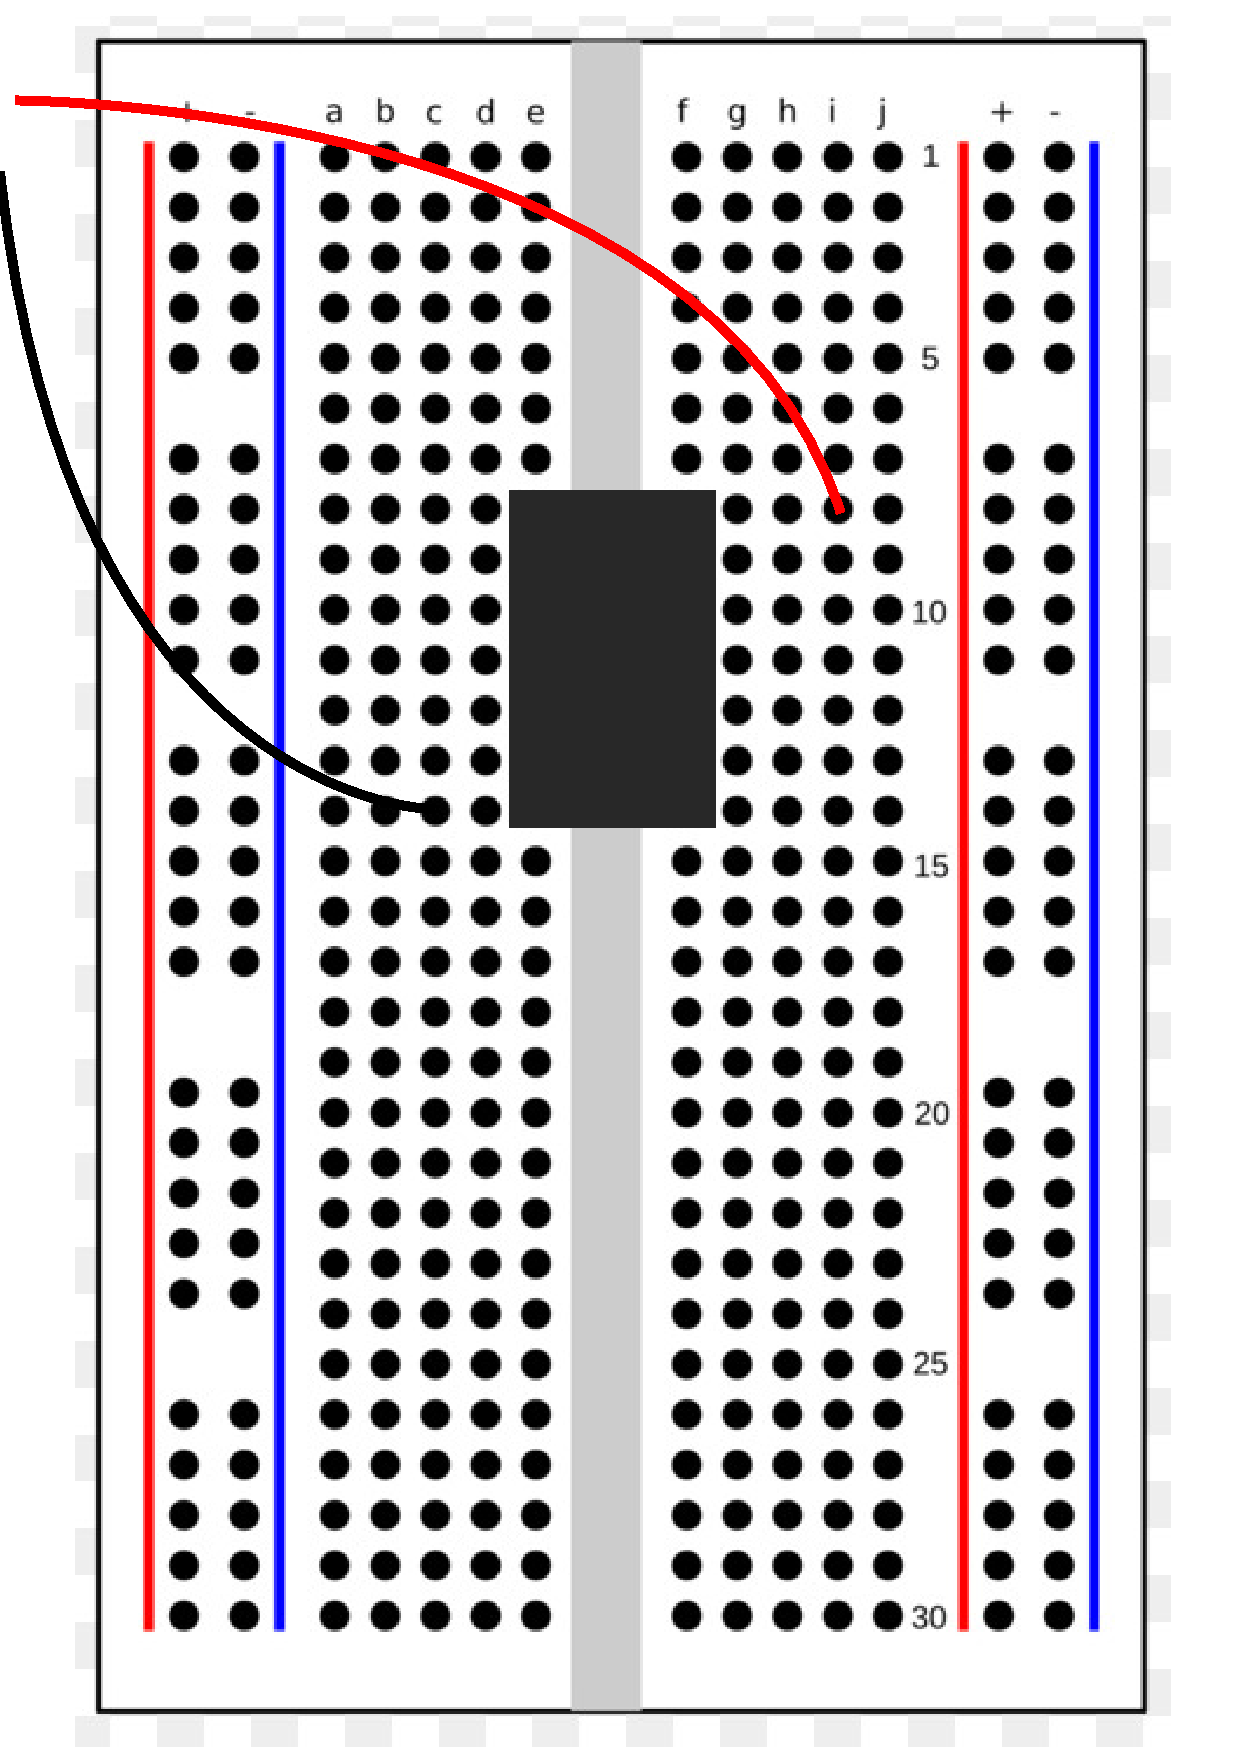
\includegraphics[width=0.37\textwidth]{breadboard_power.pdf}
\caption{\label{fig:count2} (Left) The basic breadboard layout.  The rows of five pins are connected, but the connection does not persist across the center divide.  Outer columns of five pins are also connected. (Right) Place the IC counter across the divide, and connect $V_{\rm CC}$ to pin 1 and GND to pin 8.}
\end{figure}

\section{Generating a Clock Signal with the Oscilloscope}

Things

\section{Probing IC Counter Channels with Scope Probe}

Things

\end{document}
